\documentclass[11pt, a4paper]{article}
\usepackage[T1]{fontenc}
\usepackage[top = 1.6cm, bottom = 1.6cm, left = 1cm, right = 1.5cm]{geometry}
\usepackage{amsmath,amsfonts,amssymb}
\usepackage{indentfirst,enumitem}
\usepackage{graphicx}
\usepackage{graphics}
\usepackage[font=small,labelfont=bf]{caption}
\usepackage{subcaption}
\usepackage{multicol}
\usepackage{multirow}
\usepackage{setspace}
\usepackage{hyperref}
\usepackage{listings}
\usepackage{tabularx}
\usepackage{hyperref}
\usepackage{xcolor}
\usepackage{scrextend}
\usepackage{comment}
\usepackage{soul}
\usepackage{tikz,tkz-tab}
\usepackage{lscape}
\usepackage{float,lscape}
\usepackage{fancyhdr}
\usepackage{tcolorbox}
\usepackage{titling}
\usepackage{import}
\usepackage{titlesec}
\usepackage{color}
\usepackage{empheq}

\setlength{\columnseprule}{1pt}
\def\columnseprulecolor{\color{black}}

\renewcommand\thesection{\arabic{section}}
\renewcommand\thesubsection{\arabic{section}.\arabic{subsection}}

\hypersetup{
    colorlinks=true,% make the links colored
}

\newcolumntype{M}[1]{>{\centering\arraybackslash}m{#1}}
\newcolumntype{N}{@{}m{0pt}@{}}

\pagestyle{fancy}
\fancyhead[r]{Nhat Huy}
\fancyhead[c]{\bfseries DSP}
\fancyhead[l]{\today}
\renewcommand{\headrulewidth}{0.2pt}
\setlength{\headheight}{15pt}

\begin{document}


\begin{titlepage}
    \centering
    \vspace*{1in}

    {\LARGE \bfseries Digital Signal Processing}\\[1.5cm]
    \begin{figure}[h!]
        \centering
        
\includegraphics[width=0.2\linewidth]{EE.png} $\quad$
        
\includegraphics[width=0.2\linewidth]{HCMUT.png}
    \end{figure}
    {\large Vu Nhat Huy}\\[0.5cm]
    {\large Faculty of Electrical and Electronics Engineering}\\
    {\large Department of Telecommunications Engineering}\\
    {\large Ho Chi Minh City University of Technology}\\
    {\large Contact: \href{mailto:huy.vunhat108@hcmut.edu.vn}{\it huy.vunhat108@hcmut.edu.vn}}\\[2cm]

    \vfill
    {\large Ho Chi Minh city - Ngay 29 thang 8 nam 2025}
\end{titlepage}
{
  \hypersetup{linkcolor=[RGB]{236, 16, 145}}
  \tableofcontents
  \thispagestyle{empty}
}
\newpage
\setcounter{page}{1}
%%%%%%%%%%%%%%%%%%%%%%%%%%%%%%%%%%%%%%%%%%%%%%%%%%%%%%% CHAPTER 1
\textit{\textbf{Sampling}} is to convert a continuous time signal into a discrete time signal. The analog signal is periodically measured at every T seconds.
\begin{figure}[h!]
    \centering
    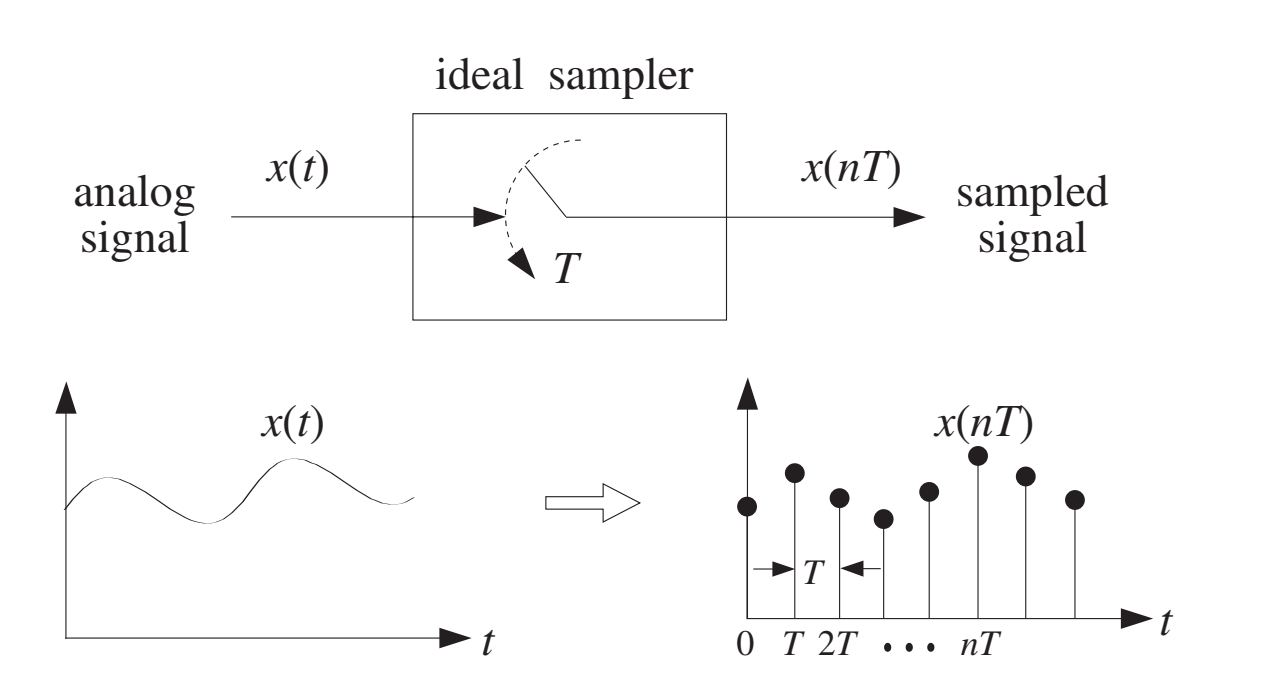
\includegraphics[width=0.5\linewidth]{img/3.png}
\end{figure}
\begin{equation*}
    x(n) \equiv x(nT)=x(t=nT),\ n=…-2, -1, 0, 1, 2, 3…
\end{equation*}
\begin{itemize}
    \item T: sampling interval or sampling period (second);
    \item Fs=1/T: sampling rate or frequency (samples/second or Hz)
\end{itemize}

\textit{\textbf{Aliasing of Sinusoids}} In general, the sampling of a continuous-time sinusoidal signal $x(t) = A\cos(2\pi F_0 t + \theta)$ at a sampling rate $ F_s=1/T $ results in a discrete-time signal $x(n)$.

The sinusoids $x_k(t) = A\cos(2\pi F_k t + \theta)$ is sampled at $F_s$, resulting  in a discrete time signal $x_k(n)$.

If $F_k=F_0+kF_s, k=0, \pm 1, \pm 2, ….,$ then $x(n)=x_k(n)$.

\textit{\textbf{Sampling Theorem}} For accurate representation of a signal $x(t)$ by its time samples $x(nT)$, two conditions must be met:
\begin{itemize}
    \item[1)] The signal $x(t)$ must be band-limited, i.e., its frequency spectrum must be limited to $F_{\max}$.
    \item[2)] The sampling rate $F_s$ must be chosen at least twice the maximum frequency $F_{\max}$. $F_s \geq 2F_{\max}$
    \begin{itemize}
        \item $F_s=2F_{\max}$ is called Nyquist rate.
        \item $F_s/2$ is called Nyquist frequency.
        \item $[-F_s/2, F_s/2]$ is Nyquist interval.
    \end{itemize}
\end{itemize}
\begin{figure}[h!]
    \centering
    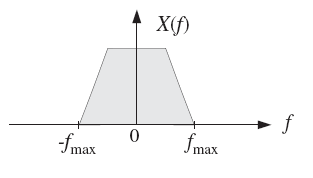
\includegraphics[width=0.3\linewidth]{img/7.png}
    \caption{Typical band-limited spectrum}
\end{figure}

\textit{\textbf{Practical antialiasing prefilter}} 
\begin{itemize}
    \item A lowpass filter: Passband $[-F_{pass}, F_{pass}]$ is the frequency range of interest for the application $(F_{max}=F_{pass})$.
    \item The stopband frequency $F_{stop}$ and the minimum stopband attenuation Astop dB must be chosen appropriately to minimize the aliasing effects.
    \item The Nyquist frequency $F_s/2$ is in the middle of transition region.
    \begin{equation*}
        F_s = F_{pass}+F_{stop}
    \end{equation*}
    \item The attenuation of the filter in decibels is defined as (where $f_0$ is a convenient reference frequency, typically taken to be at DC for a lowpass filter):
    \begin{equation*}
        A(F) = -2\log_{10}\left|\dfrac{H(F)}{H(F_0)} \right| \quad (dB)
    \end{equation*}
    \item \textbf{$\alpha_{10} =A(10F)-A(F)$ (dB/decade)}: the increase in attenuation when F is changed by a factor of ten.
    \item \textbf{$\alpha_2 =A(2F)-A(F)$ (dB/octave)}: the increase in attenuation when F is changed by a factor of two.
\end{itemize}
\begin{figure}[h!]
    \centering
    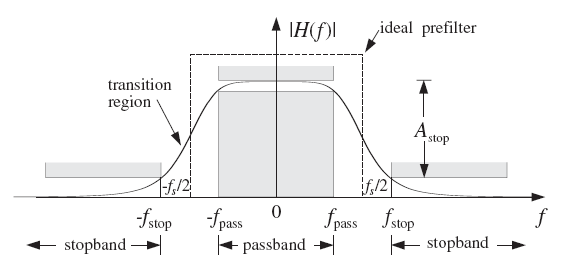
\includegraphics[width=0.5\linewidth]{img/11.png}
\end{figure}

%%%%%%%%%%%%%%%%%%%%%%%%%%%%%%%%%%%%%%%%%%%%%%%%%%%%%%% CHAPTER 2
\textit{\textbf{Quantization process}}
\begin{figure}[h!]
    \centering
    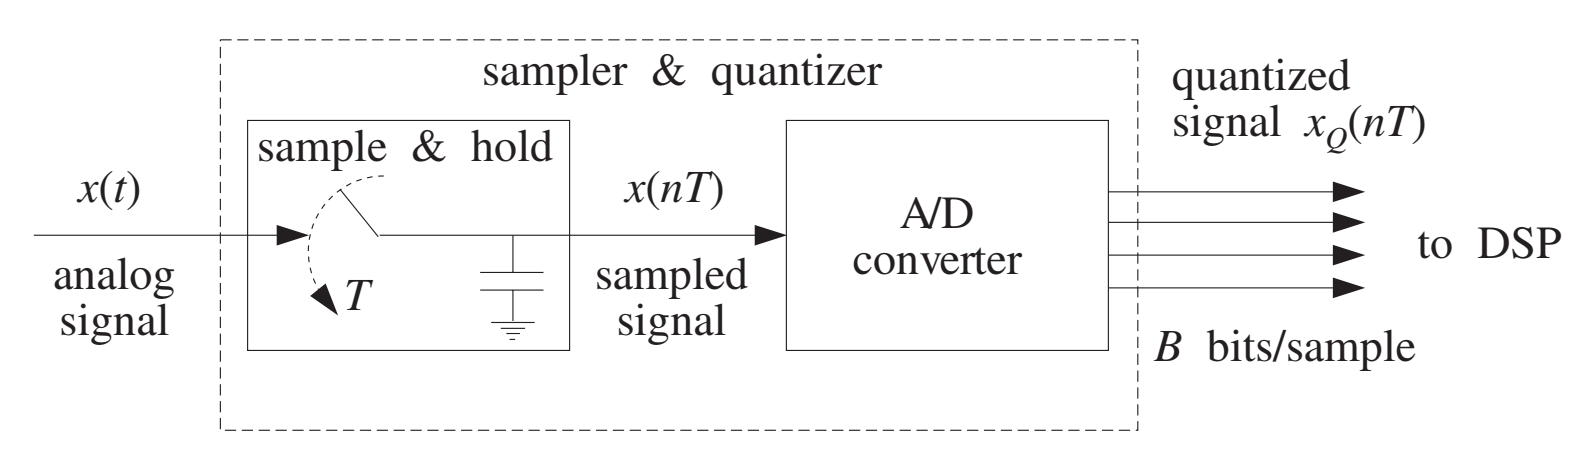
\includegraphics[width=0.5\linewidth]{img/17.png}
    \caption{Analog to digital conversion}
\end{figure}
The quantized sample $x_Q(nT)$ is represented by \textbf{B bit}, which can take $2^B$ possible values. 

An A/D is characterized by a \textbf{full-scale range R} which is divided into $2^B$ quantization levels. Typical values of R in practice are between 1-10 volts.
\begin{figure}[h!]
    \centering
    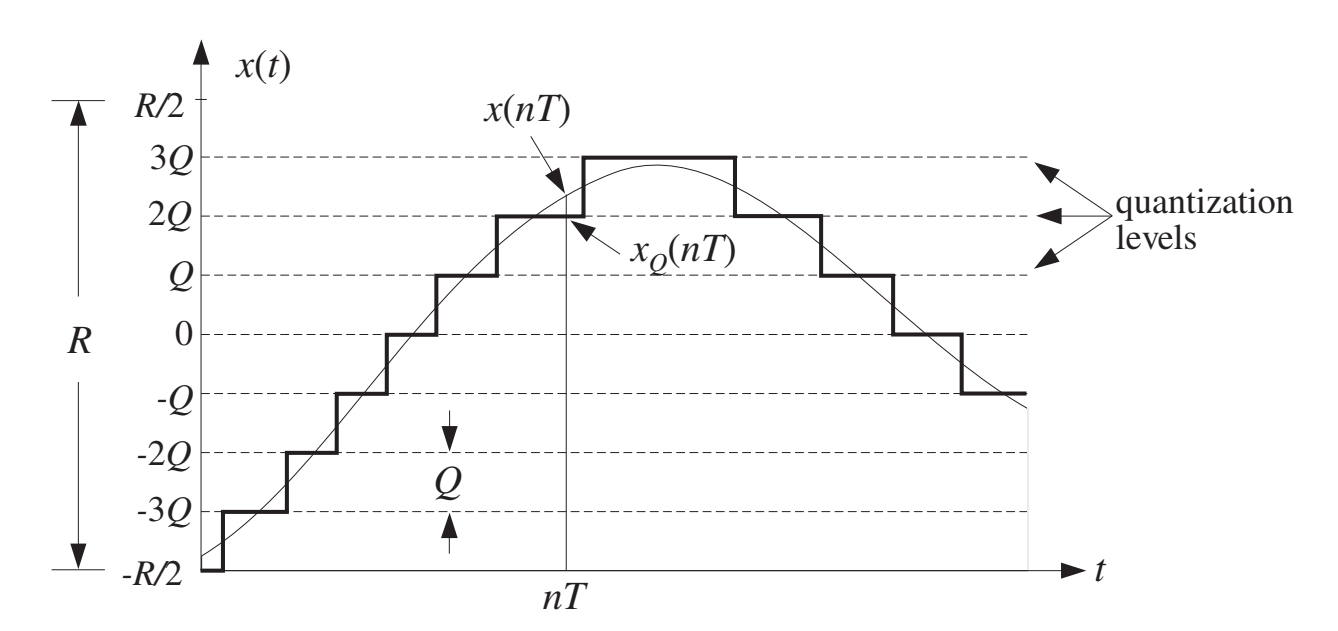
\includegraphics[width=0.5\linewidth]{img/18.png}
    \caption{Signal quantization}
\end{figure}

Quantizer resolution or quantization width (step): $Q = \dfrac{R}{2^B}$
\begin{itemize}
    \item A \textbf{bipolar} ADC: $-\dfrac{R}{2}<x_Q(nT)<\dfrac{R}{2}$
    \item A \textbf{unipolar} ADC: $0<x_Q(nT)<R$
\end{itemize}

Quantization by \textbf{\textit{rounding}}: replace each value x(nT) by the \textbf{\textit{nearest}} quantization level. 

Quantization by \textbf{\textit{truncation}}: replace each value x(nT) by its \textbf{\textit{below nearest}} quantization level.

Quantization error: $e(nT) = x_Q (nT) - x(nT)$. Consider rounding quantization: $-\dfrac{Q}{2}<e<\dfrac{Q}{2}$
\begin{figure}[h!]
    \centering
    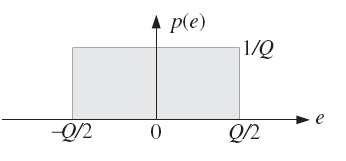
\includegraphics[width=0.3\linewidth]{img/19.png}
    \caption{Uniform probability density of quantization error}
\end{figure}

Root-mean-square (rms) error: $e_{rms}=\sigma_q=\sqrt{\overline{e^2}}=\dfrac{Q}{\sqrt{12}}$

R and Q are the ranges of the signal and quantization noise, then the \textbf{signal to noise ratio (SNR)} or \textbf{dynamic range} of the quantizer is defined as
\begin{equation*}
    SNR_{dB} = 10\log_{10}\left(\frac{\sigma^2_x}{\sigma^2_q}\right)=20\log_{10}\left(\frac{R}{Q}\right)=20\log_{10}(2^B)=6B\ dB
\end{equation*}
which is referred to as \textbf{6 dB bit rule.}

\textit{\textbf{Digital to Analog Converters (DACs)}}

\begin{figure}[h!]
    \centering
    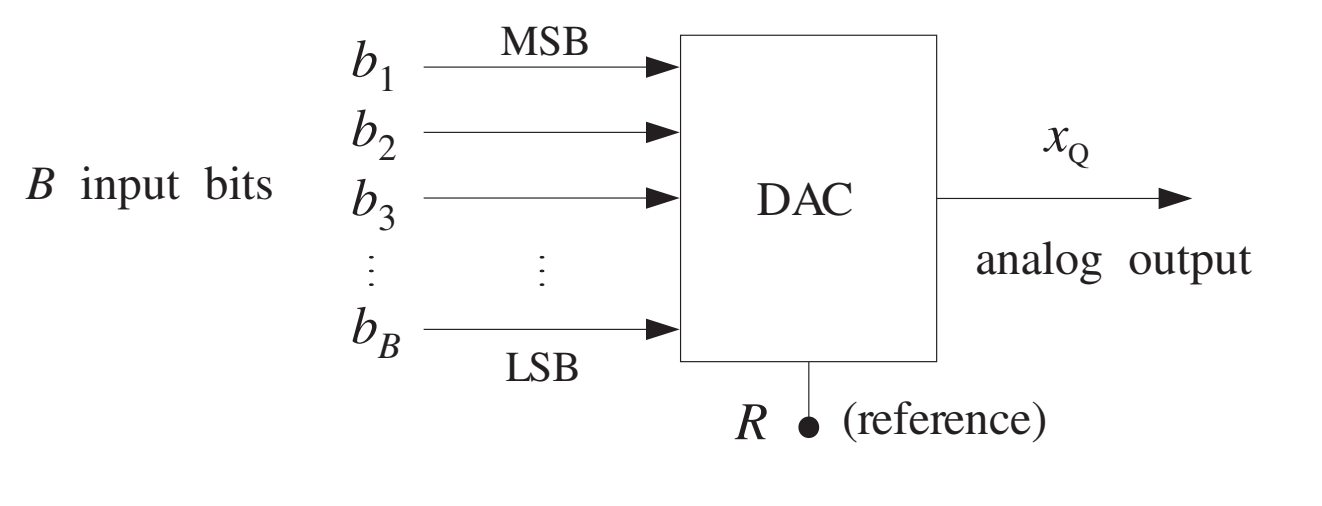
\includegraphics[width=0.5\linewidth]{img/20.png}
    \caption{B-bit D/A converter}
\end{figure}
Vector B input bits: $b=[b_1, b_2,…,b_B]$. Note that $b_B$ is the least significant bit (LSB) while $b_1$ is the most significant bit (MSB).

For unipolar signal, $x_Q \in [0, R)$; for bipolar $x_Q \in [-R/2, R/2)$.
\begin{itemize}
    \item \textbf{\textit{Unipolar natural binary}} $x_Q=R(b_12^{-1}+b_22^{-2}+...+b_B2^{-B})=Qm$ where m is the integer whose binary representation is $b=[b_1, b_2,…,b_B]$.
    \begin{equation*}
        m = b_12^{B-1}+b_22^{B-2}+...+b_B2^{0}
    \end{equation*}
    \item \textbf{\textit{Bipolar offset binary}}: obtained by shifting the $x_Q$ of unipolar natural binary converter by half-scale R/2:
    \begin{equation*}
        x_Q = R(b_12^{-1}+b_22^{-2}+...+b_B2^{-B})-\dfrac{R}{2}=Qm-\dfrac{R}{2}
    \end{equation*}
    \item \textbf{\textit{Two’s complement code}}: obtained from the offset binary code by complementing the most significant bit, i.e., replacing $b_1$ by $\overline{b_1}=1-b_1$.
    \begin{equation*}
         x_Q = R(\overline{b}_12^{-1}+b_22^{-2}+...+b_B2^{-B})-\dfrac{R}{2}
    \end{equation*}
\end{itemize}

\textit{\textbf{A/D converters}}

A/D converters quantize an analog value x so that is is represented by B bits  $b=[b_1, b_2,…,b_B]$
\begin{figure}[h!]
    \centering
    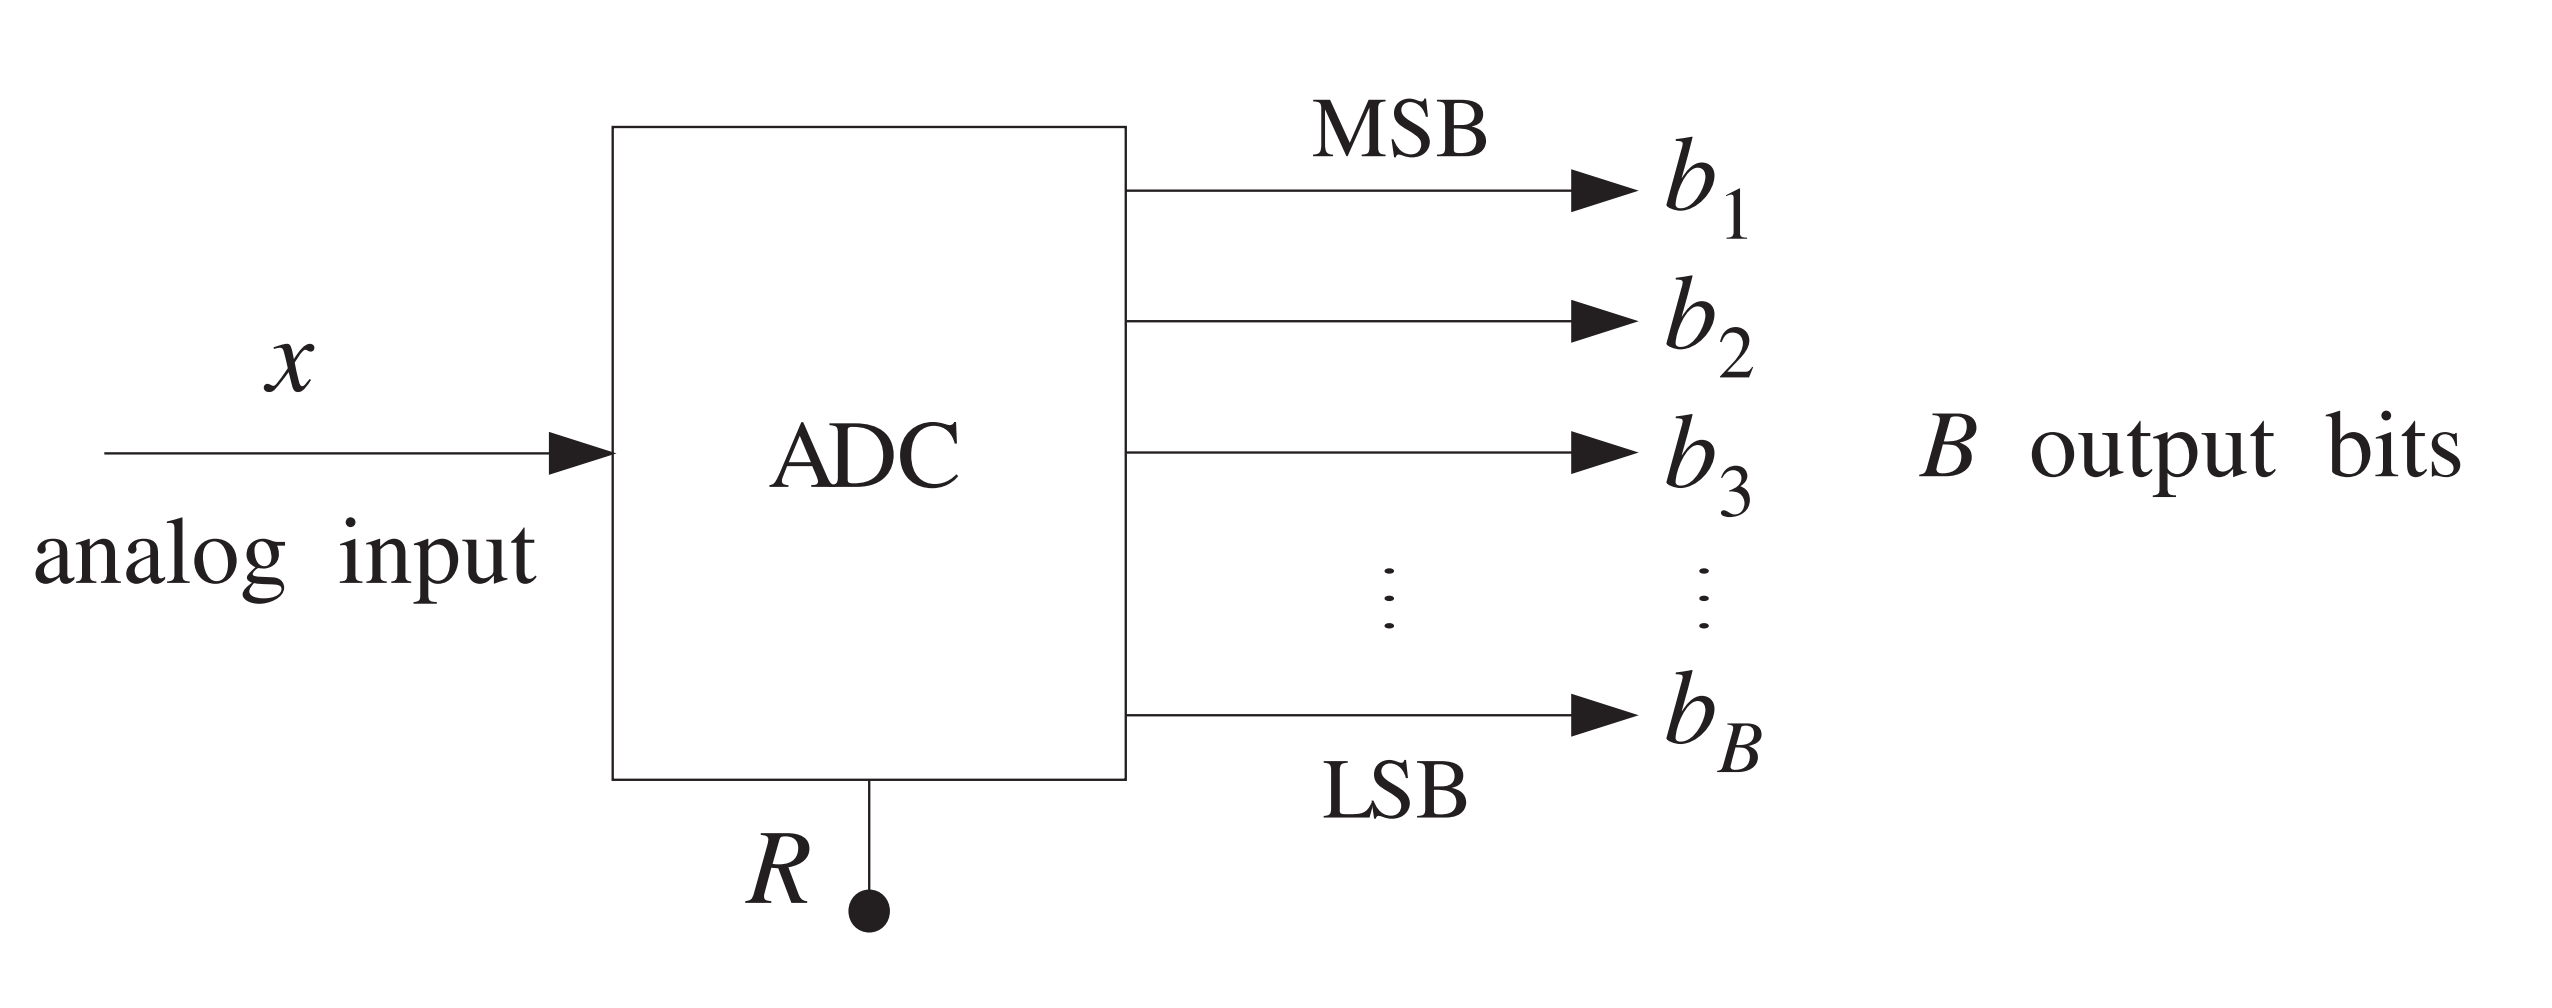
\includegraphics[width=0.4\linewidth]{img/21.png}
    \caption{B-bit A/D converter}
\end{figure}
\newpage
One of the most popular converters is the successive approximation A/D converter
\begin{figure}[h!]
    \centering
    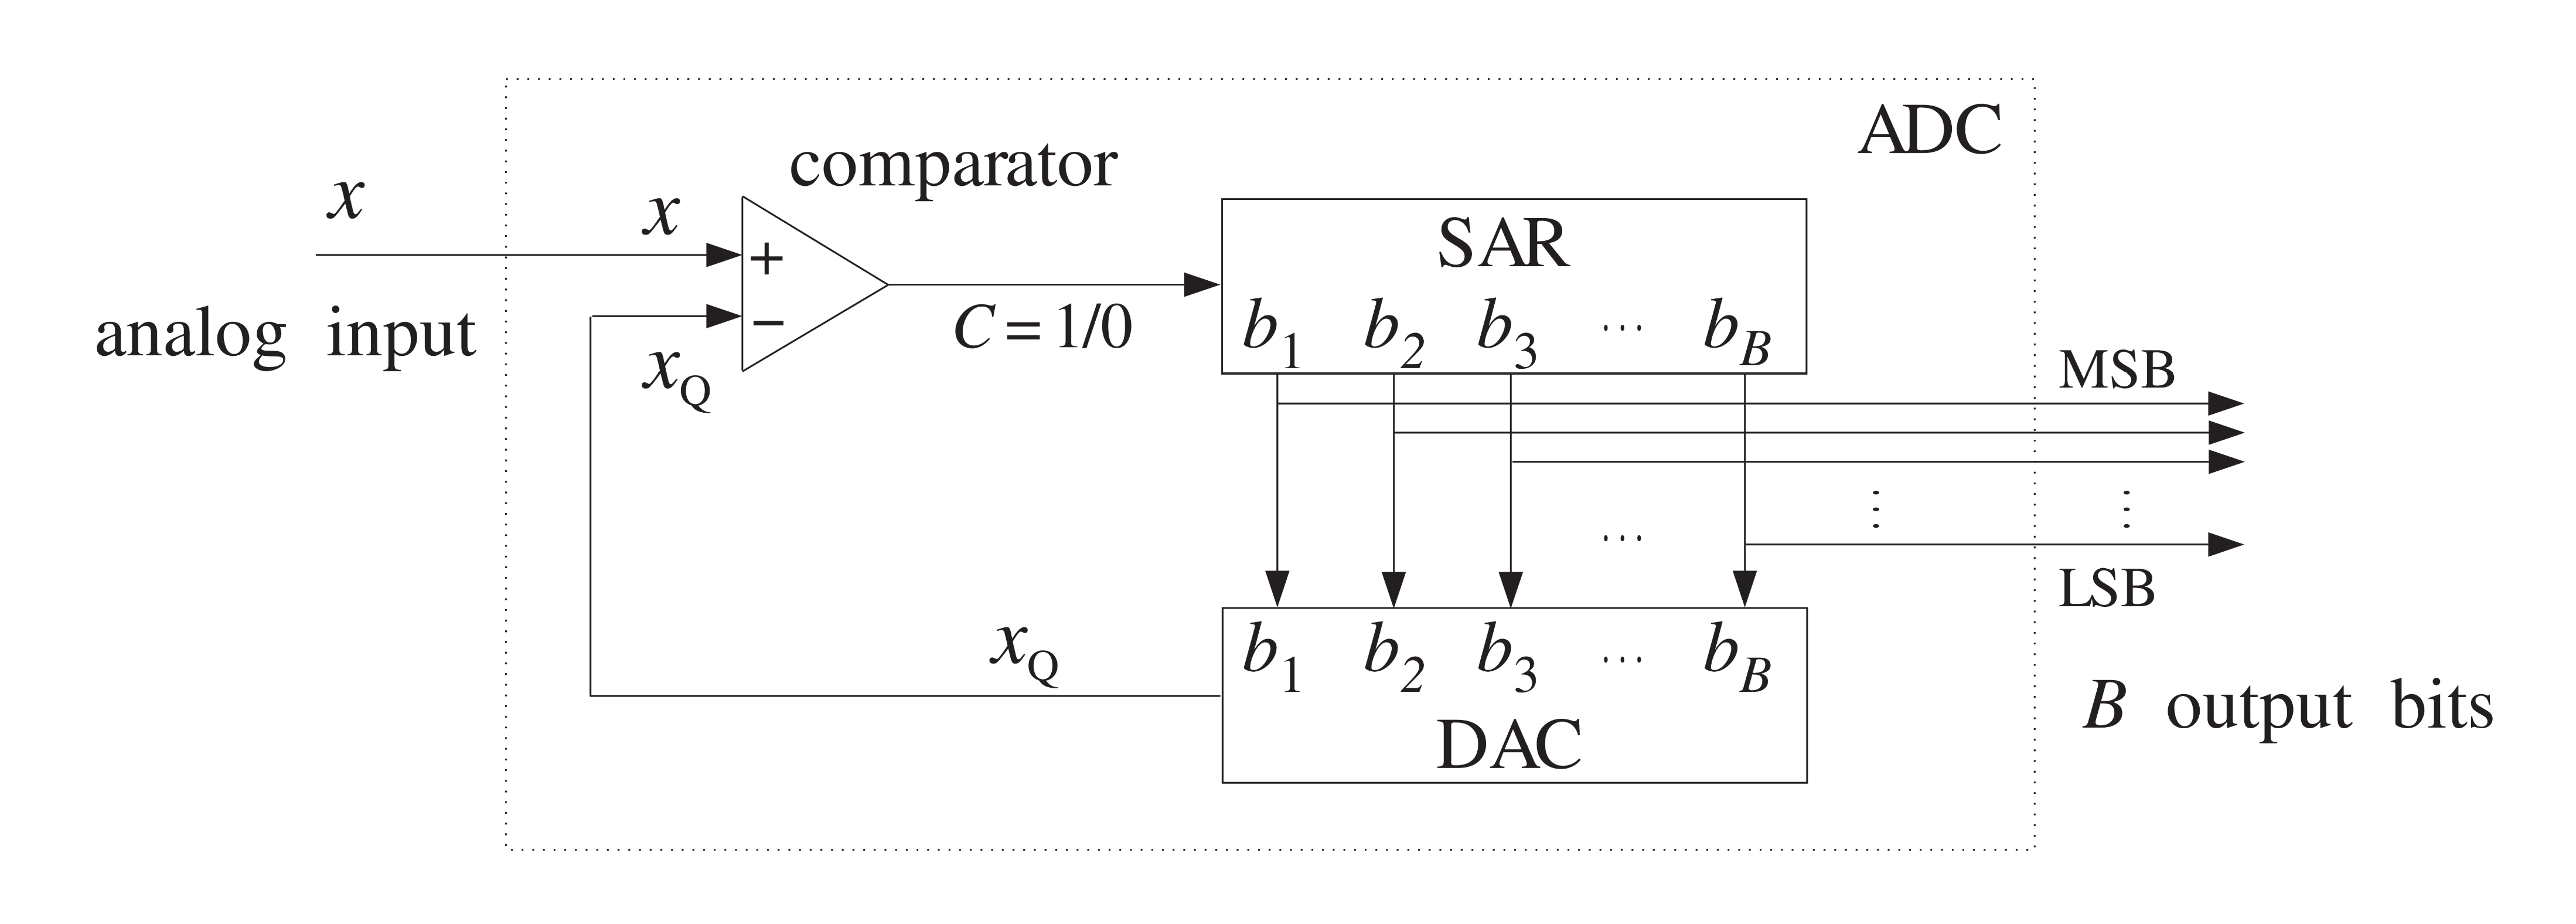
\includegraphics[width=0.5\linewidth]{img/22.png}
    \caption{Successive approximation A/D converter}
\end{figure}

After B tests, the \textbf{successive approximation register (SAR)} will hold the correct bit vector b.

\begin{figure}[h!]
    \centering
    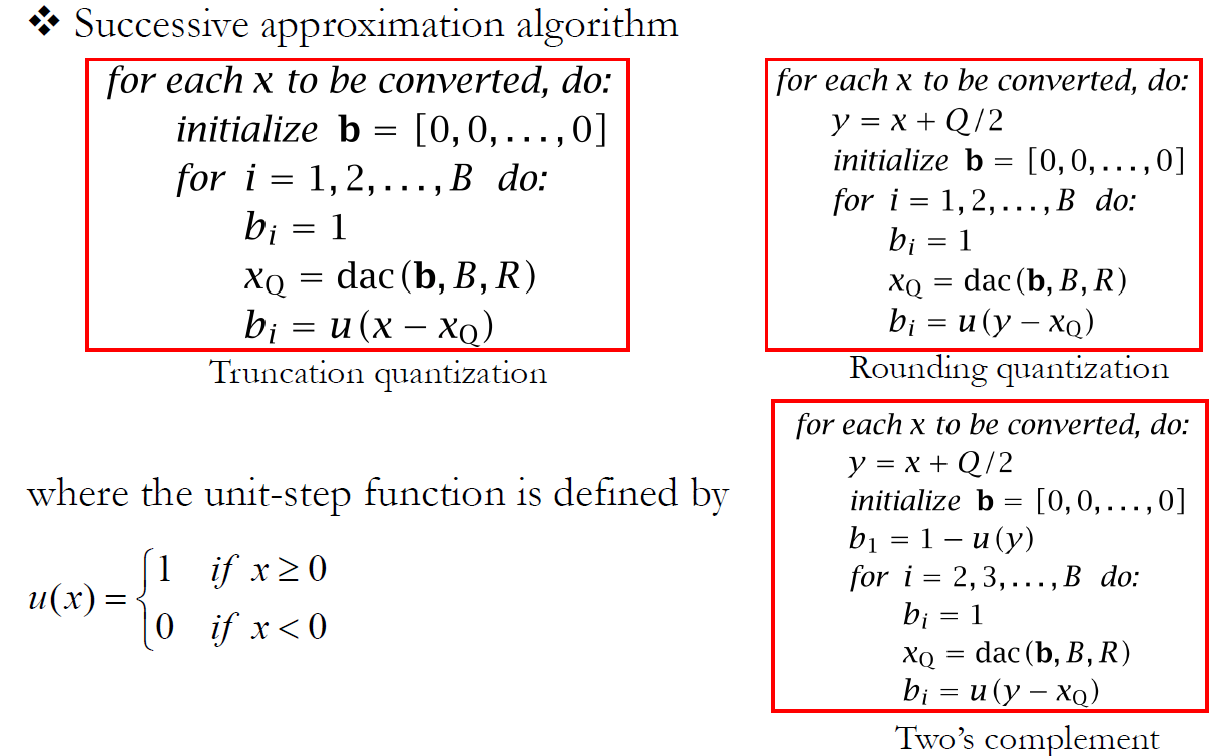
\includegraphics[width=0.5\linewidth]{img/23.png}
\end{figure}
\begin{figure}[h!]
    \centering
    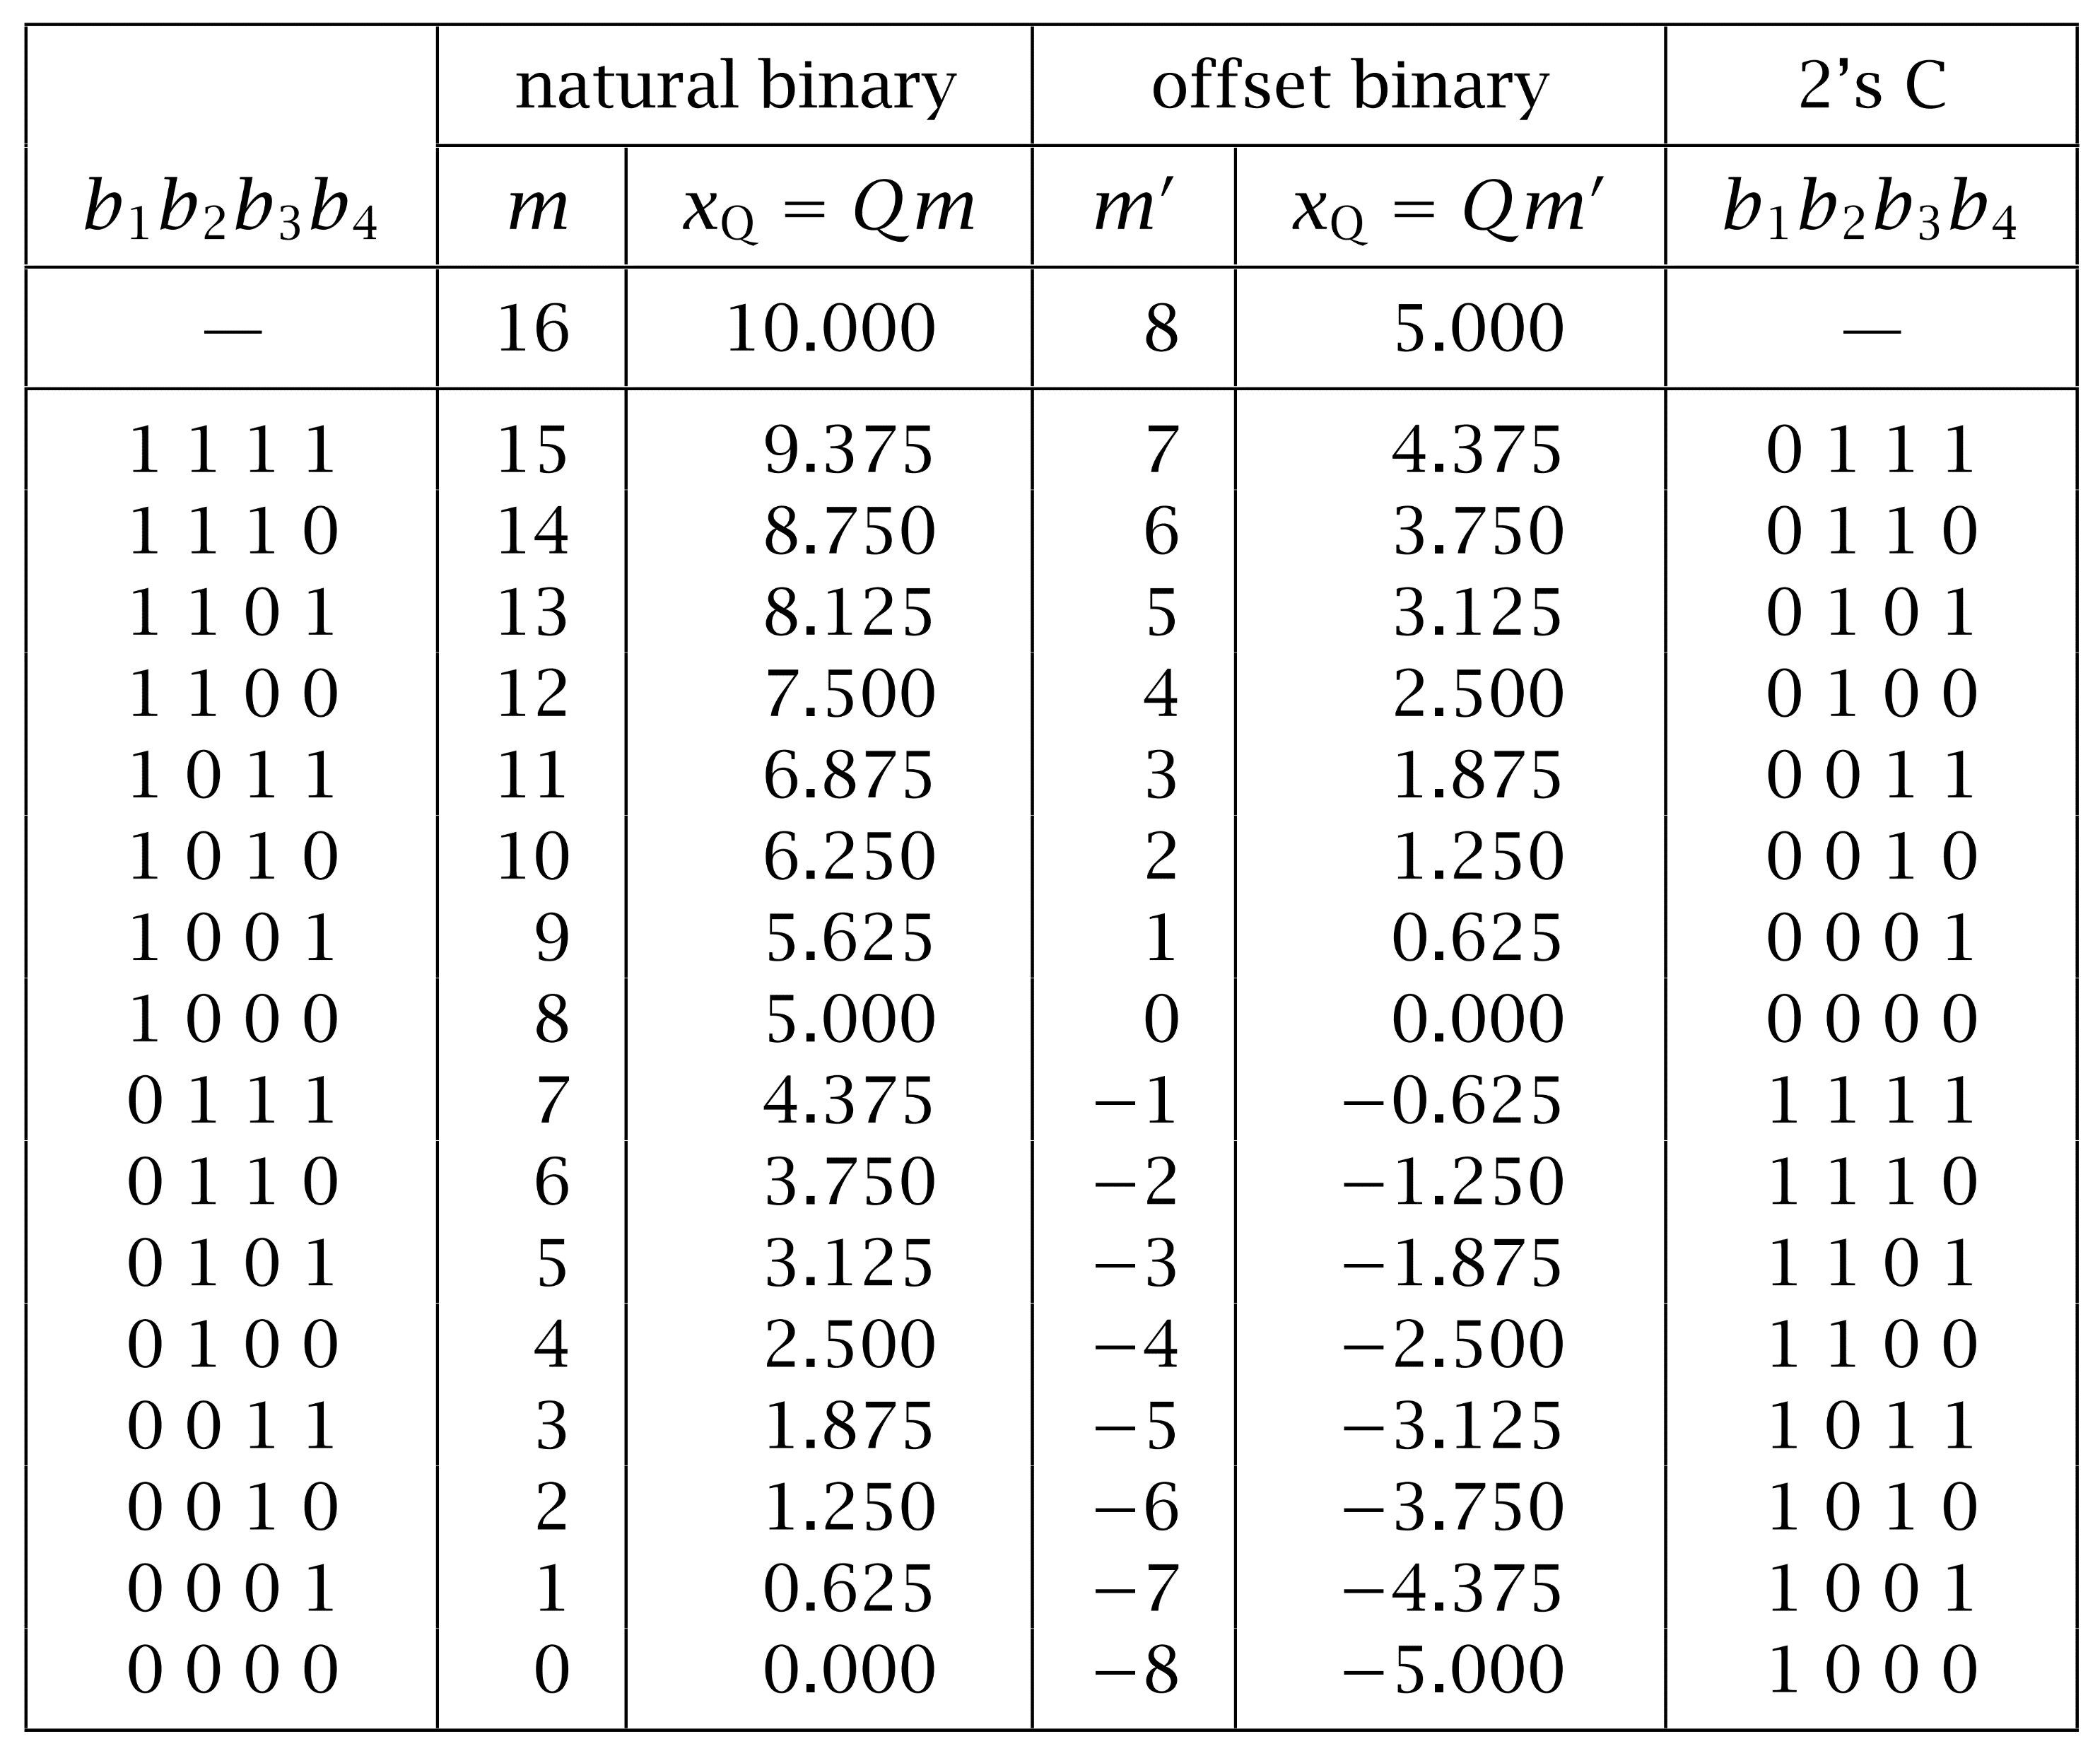
\includegraphics[width=0.5\linewidth]{img/28.png}
    \caption{Converter codes for B = 4 bits, R = 10 volts}
\end{figure}

%%%%%%%%%%%%%%%%%%%%%%%%%%%%%%%%%%%%%%%%%%%%%%%%%%%%%%% CHAPTER 3
Unit sample sequence (unit impulse): $\displaystyle \delta(n) \begin{cases}
    1 \quad for\ n=0 \\
    0 \quad for\ n\neq 0
\end{cases} $

Unit step signal: $\displaystyle \delta(n) \begin{cases}
    1 \quad for\ n\geq 0 \\
    0 \quad for\ n< 0
\end{cases} $

\textbf{\textit{Input/output rules}}.

A discrete-time system is a processor that transform an input sequence $x(n)$ into an output sequence $y(n)$.
\begin{figure}[h!]
    \centering
    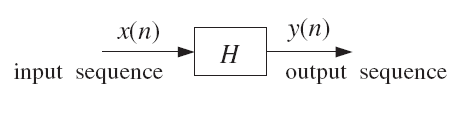
\includegraphics[width=0.4\linewidth]{img/29.png}
    \caption{Discrete-time system}
\end{figure}\\
Sample-by-sample processing: $\{x_0,x_1,x_2,...,x_n\} \xrightarrow{H} \{y_0,y_1,y_2,...,y_n\}$ that is, $x_0 \xrightarrow{H}y_0, \ x_1 \xrightarrow{H} y_1,...$ and so on.\\
Block processing: $x = \begin{bmatrix}
    x_0 \\
    x_1 \\ 
    x_2 \\
    \vdots 
\end{bmatrix} \xrightarrow{H} \begin{bmatrix}
    y_0 \\
    y_1 \\ 
    y_2 \\
    \vdots 
\end{bmatrix}=y$\\
\begin{figure}[h!]
    \centering
    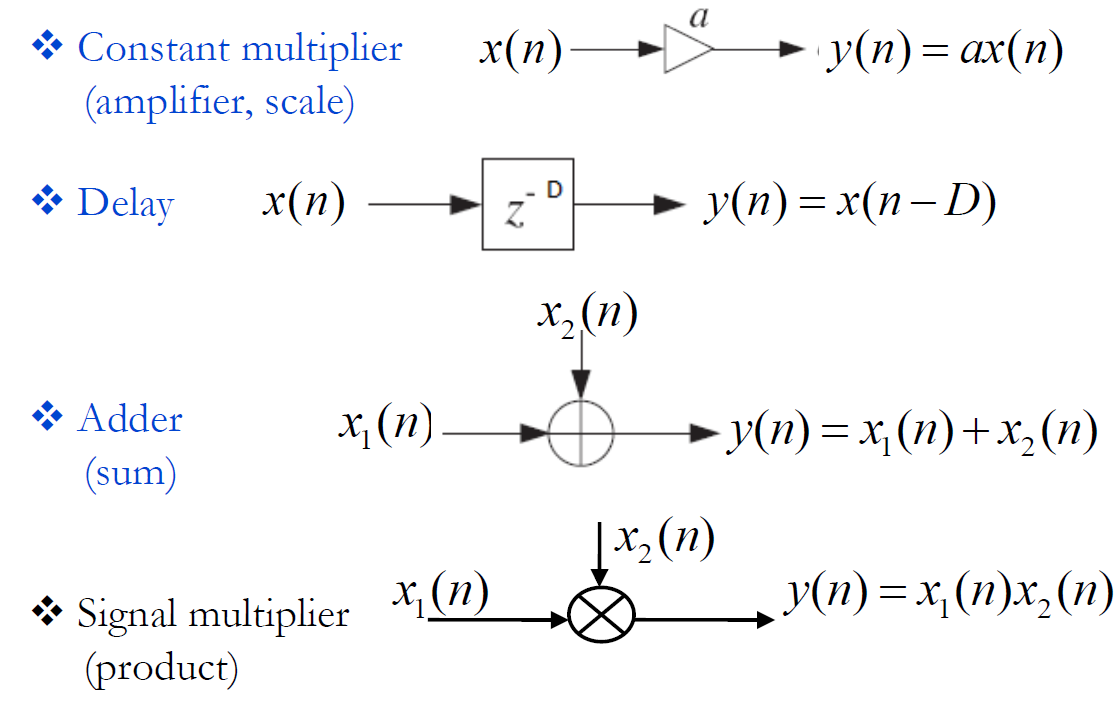
\includegraphics[width=0.5\linewidth]{img/30.png}
    \caption{Basic building blocks of DSP systems}
\end{figure}

\textbf{\textit{Linearity and time invariance}}

A \textbf{linear system} has the property that the output signal due to a linear combination of two input signals can be obtained by forming the same linear combination of the individual outputs.
\begin{figure}[h!]
    \centering
    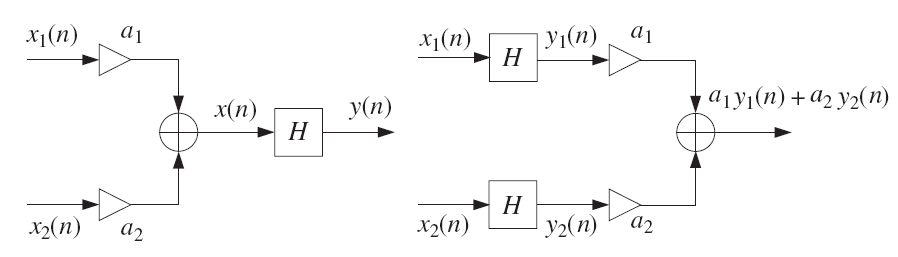
\includegraphics[width=0.6\linewidth]{img/31.png}
    \caption{Testing linearity}
\end{figure}

If $x(n)=a_1x_1(n)+a_2x_2(n) \to y(n)=a_1y_1(n)+a_2y_2(n) \ \forall a_1,a_2 \to$ linear system. Otherwise, the system is nonlinear.
\newpage
A \textbf{time-invariant system} is a system that its input-output characteristics do not change with time.
\begin{figure}[h!]
    \centering
    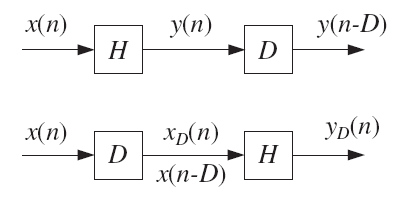
\includegraphics[width=0.5\linewidth]{img/32.png}
    \caption{Testing time invariance}
\end{figure}

If $y_D(n)=y(n-D) \ \forall D \to$ time-invariant system. Otherwise, the system is time-variant.

\textbf{\textit{Impulse repsonse}}

\textbf{Linear time-invariant (LTI) systems} are characterized uniquely by their impulse response sequence $h(n)$, which is defined as the response of the systems to a unit impulse $\delta(n)$.
\begin{figure}[h!]
    \centering
    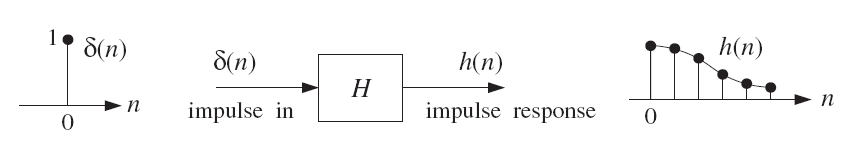
\includegraphics[width=0.5\linewidth]{img/33.png}
    \caption{Impulse response of an LTI system}
\end{figure}
\begin{figure}[h!]
    \centering
    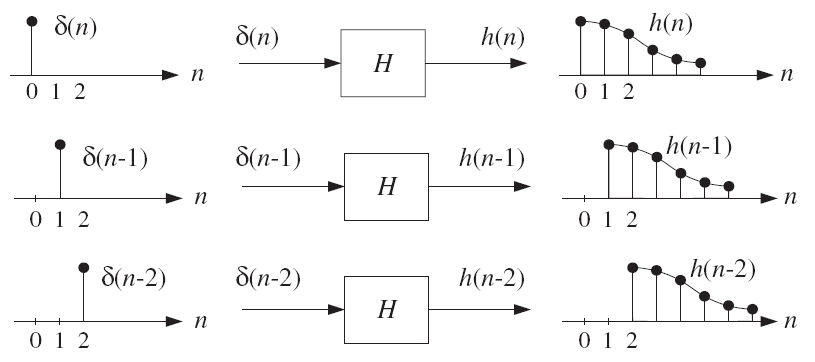
\includegraphics[width=0.5\linewidth]{img/34.png}
    \caption{Delayed impulse response of an LTI system}
\end{figure}

A \textbf{finite impulse response (FIR) filter} has impulse response $h(n)$ that extend only over a finite time interval, say $0 \leq n \leq M$.
\begin{figure}[h!]
    \centering
    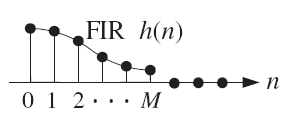
\includegraphics[width=0.3\linewidth]{img/35.png}
    \caption{FIR impulse response}
\end{figure}
\begin{itemize}
    \item $M$: filter order; $L_h=M+1$: the length of impulse response.
    \item $h=\{h_0,\ h_1,\ ...,\ h_M\}$ is referred by varius name such as filter coefficients, filter weights or filter taps.
    \item FIR filtering equation: $y(n) = \displaystyle\sum_{m=0}^{M}h(m)x(n-m)=h(n)*x(n) $
\end{itemize}
\newpage
A \textbf{infinite impulse response (IIR) filter} has impulse response $h(n)$ of infinite duration, say $0\leq n \leq\infty$.
\begin{figure}[h!]
    \centering
    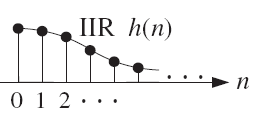
\includegraphics[width=0.3\linewidth]{img/36.png}
    \caption{IIR impulse response}
\end{figure}

IIR filtering equation: $y(n) = \displaystyle\sum_{m=0}^{M}h(m)x(n-m)=h(n)*x(n) $. The I/O equation of IIR filters are expressed as the recursive differences equation.

\textit{\textbf{Causality and Stability}}

\begin{figure}[h!]
    \centering
    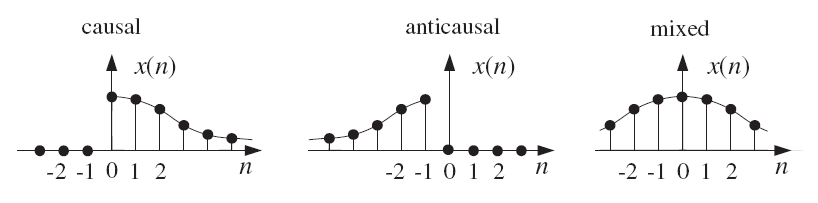
\includegraphics[width=0.5\linewidth]{img/37.png}
    \caption{Causal, Anticasual and Mixed signals}
\end{figure}

LTI systems can also classified in terms of causality depending on whether $h(n)$ is casual, anticausal or mixed. A system is stable (BIBO) if \textbf{bounded inputs} ($|x(n)| \leq A$) always generate \textbf{bounded outputs} ($|y(n)| \leq B$).

A LTI system is stable $\Leftrightarrow \displaystyle \sum_{n=-\infty}^{\infty} (h(n))<\infty$


\end{document}